%! Author = jaggi
%! Date = 6/16/25

% Preamble
\documentclass[11pt]{article}

% Packages
\usepackage{array}
\usepackage[export]{adjustbox}
\usepackage{caption}
\usepackage[
  backend=biber,
  %style=reading
]{biblatex}
\usepackage[utf8]{inputenc}
\usepackage[T1]{fontenc}
\usepackage{hyperref}
\usepackage{graphicx}
\usepackage{geometry}
\usepackage{xcolor}
\usepackage{titlesec}
\usepackage{enumitem}
\usepackage{lmodern}
\usepackage{wasysym}
\usepackage{pgfplots}
\usepackage{svg}
\usepackage[off]{svg-extract}
\svgsetup{clean=true}
%\pdfsuppresswarningpagegroup=1
\usepackage{siunitx}
\usepackage{tikz}
\usepackage{tkz-euclide}
\usepackage[european,straightvoltages]{circuitikz}

% Define a flag depending on compiler
\newif\ifhtml
\ifdefined\HCode
\htmltrue  % We're using make4ht/tex4ht
\else
\htmlfalse % We're using pdflatex or other
\fi

\addbibresource{electronics.bib}

\title{Electronics}
\author{Jaggi the nerdy fuzzball}
\date{2025-06-19}

% Document
\begin{document}
\maketitle
\ifhtml
\begin{center}
  \vspace{2em}
  \renewcommand{\arraystretch}{1.5}
  \begin{tabular}{
      >{\raggedright\arraybackslash}p{0.3\linewidth}
      >{\raggedright\arraybackslash}p{0.3\linewidth}
      >{\raggedright\arraybackslash}p{0.3\linewidth}
    }
    \href{../../index.html}{Blog Index} &
    \href{electronics.pdf}{PDF
    Version}                            &
    \href{../../about.html}{About}              \\
    ~                                   & ~ & ~ \\
  \end{tabular}
\end{center}
\fi
\begin{flushright}
  \textit
  {Confusion will be my epitaph\\
    As I crawl, a cracked and broken path\\
    If we make it, we can all sit back and laugh\\
  But I fear tomorrow I'll be crying}\par
  King Crimson -- Epitaph -- 1969
\end{flushright}

\tableofcontents

\newpage
\begin{abstract}
  My notes about studying electronics and microwave engineering,
  intended for me first and foremost, but you're welcome to contribute.
  Beginning with the foundational principles of electricity, circuit
  theory, and passive components, then move toward more advanced
  topics in digital logic, operational amplifiers, and control systems.

  The second half extends into radio-frequency (RF) and microwave
  domains, covering key principles such as electromagnetic wave
  propagation, transmission lines, waveguides, antenna design,
  microwave components, and communication systems.

  This document is published as is, with no warranty on the accuracy
  of it's content.
\end{abstract}

\begin{table}[h!]
  \centering
  \begin{tabular}{
      >{\centering\arraybackslash}p{0.35\textwidth}
      >{\raggedright\arraybackslash}m{0.65\textwidth}
    }
    \ifdefined\HCode
    \raisebox{-0.5\totalheight}{
      
\includegraphics[height=15em,keepaspectratio]
      {src/assets/jaggi_teach.png}
    }
    \else
    \raisebox{-0.5\totalheight}{
      
\includegraphics[height=9em,keepaspectratio]
      {src/assets/jaggi_teach_full.png}
    }
    \fi
    &
    \noindent
    Ohm my gosh—I’m just amping up your learning, one electron at a time!
  \end{tabular}
\end{table}

\section{Introduction} \label{sec:introduction}

\section{Fundamental Electrical Principles} \label{sec:fundamentals}
\subsection{DC Circuit Theory} \label{subsec:dc_circuit_theory}
DC circuit theory lays the groundwork for all electronics by
describing how static (time‑invariant) voltages and currents behave
in closed loops.\\

\begin{figure}[!h]
  \centering
  \ifdefined\HCode
  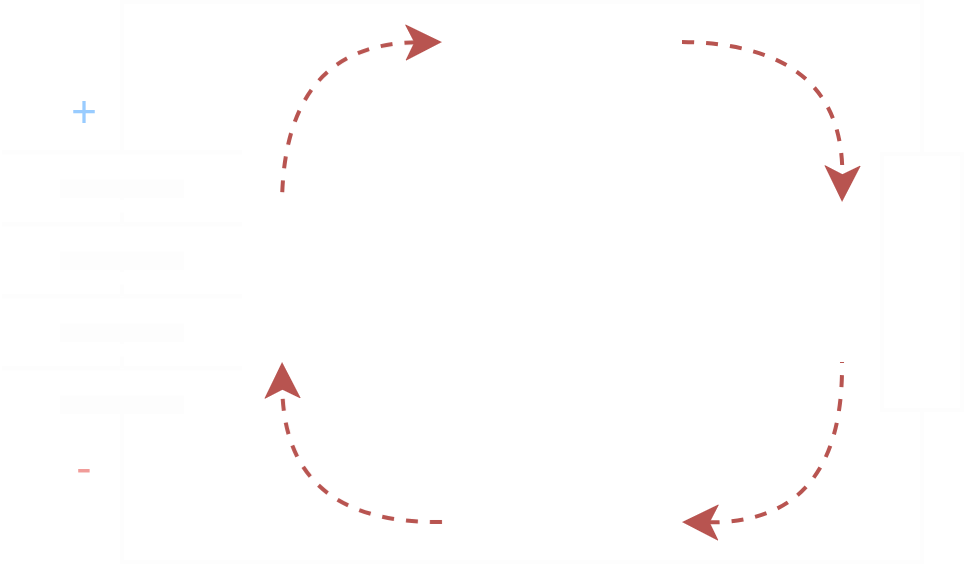
\includegraphics[height=25em,width=42em]
  {src/assets/current-flow-dark.png}
  \else
  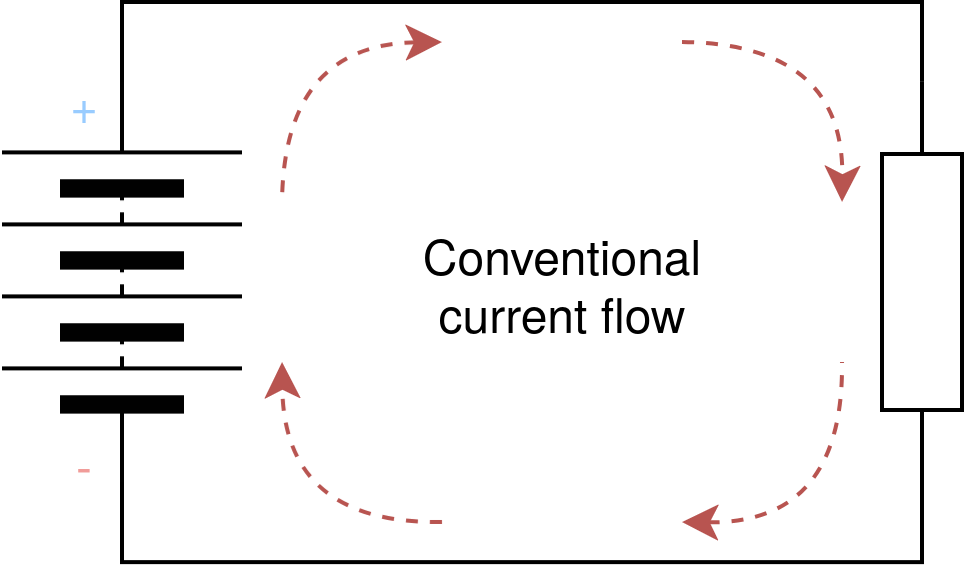
\includegraphics[width=0.5\textwidth,keepaspectratio]
  {src/assets/current-flow-light.png}
  \fi
  \caption{The conventional current flow, from \(+\) to --}
\end{figure}

\subsubsection{The units handled}

Before diving into circuits and components, it is important to define
the \textit{fundamental units} that form the language of electronics.
At the root is \textbf{electric charge}, the basic quantity underlying
all electrical interactions. From charge arises \textbf{electric
current}, the flow of charges through a conductor, and \textbf{voltage},
the potential difference that drives this flow. Materials oppose the
motion of charges through their \textbf{resistance}, while the concepts
of \textbf{energy} and \textbf{power} allow us to describe how circuits
store and deliver useful work. Together, these units establish the
framework through which we measure and analyze electrical phenomena.\par
\vspace{\baselineskip}
\textbf{\underline{Electric charge :}}\par
\noindent
Electric charge is a fundamental property of matter, it enables
interactions via electromagnetic fields. It is quantified in \textbf{coulombs
(\unit{\coulomb})}. There are two kinds of electric charge, labelled as
positive and negative. Like charges repel, whereas opposite charges
attract. In ordinary matter, the total of positive and negative
charges is balanced, a condition known as electrical neutrality.
Electrons (--) and protons (\(+\)) serve as the principal carriers of
electric charge.

\begin{figure}[!h]
  \centering
  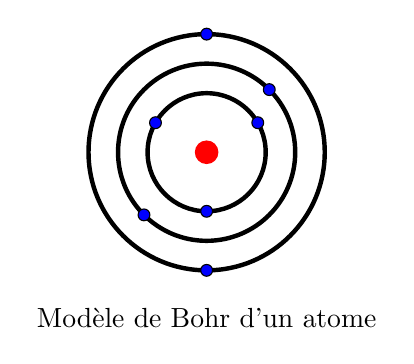
\begin{tikzpicture}[scale=0.75]
    \fill[red] (0,0) circle (0.2);
    \draw[ultra thick] (0,0) circle (1);
    \draw[ultra thick] (0,0) circle (1.5);
    \draw[ultra thick] (0,0) circle (2);
    \foreach \theta in {30, 150, 270}
    \draw[fill=blue] (\theta:1) circle (0.1);

    \foreach \theta in {45, 225}
    \draw[fill=blue] (\theta:1.5) circle (0.1);

    \foreach \theta in {90, 270}
    \draw[fill=blue] (\theta:2) circle (0.1);
    \node[below=1em] at (0, -2) {Modèle de Bohr d'un atome};
  \end{tikzpicture}
\end{figure}

In industrial and engineering contexts, the ampere‑hour (Ah)—and its
submultiples—is commonly used in lieu of the coulomb, particularly
when indicating the capacity of a battery, in which case:
\[
  1~\unit{\ampere\hour} = 3\,600~\unit{\coulomb}.
\]
This unit makes it straightforward to estimate how long a battery can
sustain a given current; for instance, a 30\unit{\ampere\hour} battery
delivering 1\unit{\ampere}
would theoretically last 30\unit{\hour} (or 15\unit{\hour} at
2\unit{\ampere}), and so
on.

\textbf{Key properties of electric charge (Coulomb’s law):}
\begin{enumerate}
  \item There are two types of charge: positive and negative.
  \item Charges of the same type repel one another.
  \item Charges of opposite types attract one another.
\end{enumerate}

An electric current is the collective motion of charged
carriers—typically electrons—through a conductive medium, driven by
the electromagnetic force. It is expressed in amperes (\unit{\ampere}),
which corresponds to the passage of one coulomb of charge per
second.

\subsubsection{Ohm's Law and Power}
text\par
\begin{figure}[!h]
  \centering
  \ifdefined\HCode
  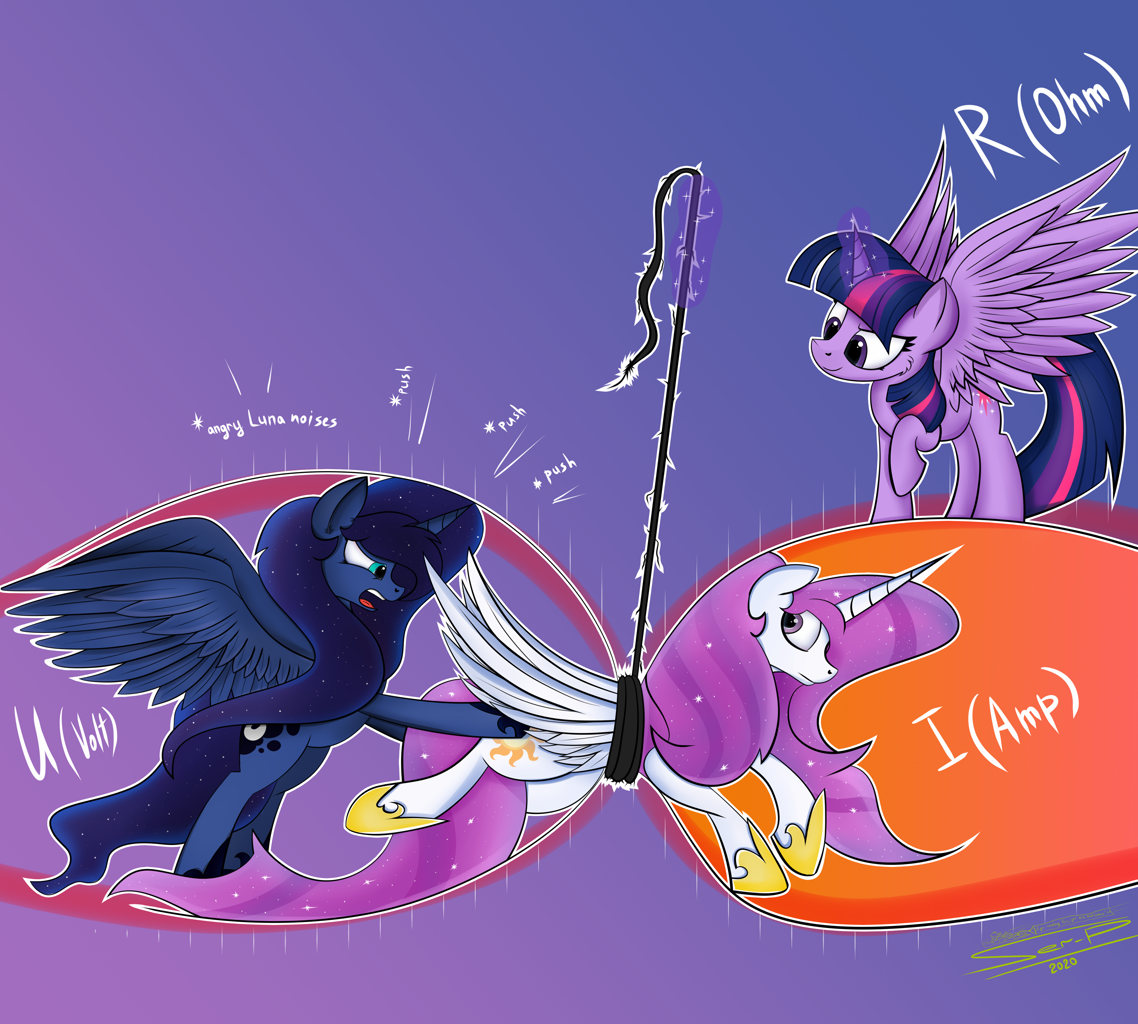
\includegraphics[height=45em,keepaspectratio]
  {src/assets/electricity_pony.png}
  \else
  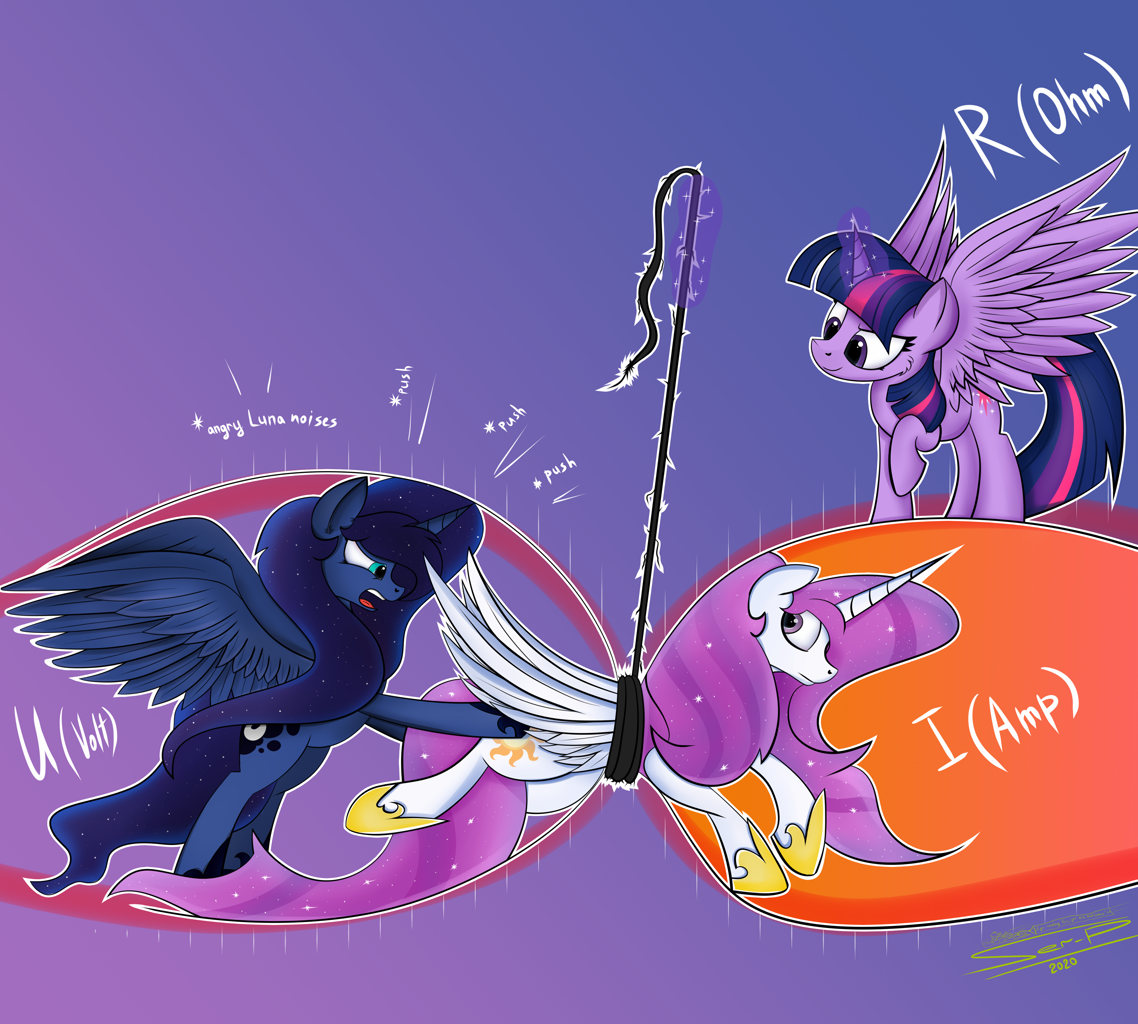
\includegraphics[height=0.7\textwidth,keepaspectratio]
  {src/assets/electricity_pony.png}
  \fi
  \caption{Electrical resistance explained with ponies.\\
    \textbf{Source:}\href{
      https://derpibooru.org/images/2461820?q=electrical+resistance
    }{
      derpibooru.org
    }
  }
\end{figure}
\subsection{Basic Components} \label{subsec:basic_components}
\subsubsection{Resistors}
\subsubsection{Capacitors}
\subsubsection{Inductors (Coil Inductance, Magnetic Flux)}
\subsubsection{Diodes}
\subsubsection{Transistors}
\subsection{Schematics and Symbols} \label{subsec:schematics_symbols}

\section{Analog and AC Circuits} \label{sec:analog_ac}
\subsection{AC Circuit Theory} \label{subsec:ac_circuit_theory}
\subsubsection{RLC Circuits}
\subsubsection{Impedance and Reactance}
\subsection{Filters and Frequency Response} \label{subsec:filters}
\subsection{Transformers and Electromagnetism} \label{subsec:transformers}
\subsection{Power Supplies and Power Electronics}
\label{subsec:power_electronics}

\section{Operational Amplifiers and Oscillators} \label{sec:opamps_oscillators}
\subsection{Operational Amplifiers} \label{subsec:opamps}
\subsubsection{Inverting and Non-Inverting Amplifiers}
\subsubsection{Feedback and Gain Control}
\subsection{Oscillators} \label{subsec:oscillators}
\subsubsection{RC Oscillators}
\subsubsection{LC Oscillators}

\section{Digital Electronics and Logic} \label{sec:digital_electronics}
\subsection{Number Systems} \label{subsec:number_systems}
\subsubsection{Binary}
\subsubsection{Hexadecimal}
\subsection{Boolean Algebra and Logic Gates} \label{subsec:boolean_logic}
\subsubsection{AND, OR, NOT, NAND, NOR Gates}
\subsection{Combinational Logic} \label{subsec:combinational_logic}
\subsubsection{Multiplexers}
\subsubsection{Encoders and Decoders}
\subsection{Sequential Logic} \label{subsec:sequential_logic}
\subsubsection{Flip-Flops}
\subsubsection{Counters}
\subsubsection{Registers}

\section{Electronic Systems and Control} \label{sec:systems_control}
\subsection{System Theory} \label{subsec:system_theory}
\subsubsection{Inputs and Outputs}
\subsubsection{Block Diagrams}
\subsection{Feedback Systems} \label{subsec:feedback}
\subsubsection{Open-Loop Control}
\subsubsection{Closed-Loop Control}

\section{Radio Frequency (RF) Foundations} \label{sec:rf_foundations}
\subsection{RF and Microwave Spectrum} \label{subsec:rf_spectrum}
\subsection{Electromagnetic Wave Propagation} \label{subsec:wave_propagation}
\subsubsection{Line-of-Sight Constraints}
\subsection{Transmission Line Basics} \label{subsec:transmission_lines}
\subsubsection{S-Parameters and dB Units}

\section{Transmission Lines and Waveguides} \label{sec:waveguides}
\subsection{Coaxial and Microstrip Lines} \label{subsec:coaxial_microstrip}
\subsection{Waveguide Theory} \label{subsec:waveguide_theory}
\subsubsection{Modes of Propagation}
\subsubsection{Cutoff Frequency}

\section{Microwave Components and Devices} \label{sec:microwave_components}
\subsection{Antennas and Resonators} \label{subsec:antennas_resonators}
\subsection{Microwave Sources} \label{subsec:microwave_sources}
\subsubsection{Klystron}
\subsubsection{Magnetron}
\subsubsection{Gunn Diode}
\subsubsection{Traveling-Wave Tube (TWT)}
\subsection{Passive Microwave Devices} \label{subsec:passive_microwave}
\subsubsection{Directional Couplers}
\subsubsection{E-Plane and H-Plane Tees}
\subsubsection{Rat-Race Junctions}

\section{Microwave Communication Systems} \label{sec:microwave_communications}
\subsection{Point-to-Point Microwave Links} \label{subsec:microwave_links}
\subsection{Satellite and Terrestrial Systems} \label{subsec:satellite_systems}
\subsection{Radar Principles} \label{subsec:radar}
\subsection{RF PCB Design Considerations} \label{subsec:rf_pcb}

\section{Microwave Measurements, Safety, and Standards}
\label{sec:microwave_measurements}
\subsection{Measurement Techniques} \label{subsec:measurement_techniques}
\subsubsection{Power, Attenuation, Phase}
\subsection{Microwave Radiation Safety} \label{subsec:microwave_safety}

\section{Advanced RF Topics} \label{sec:advanced_rf}
\subsection{Impedance Matching and Smith Chart}
\label{subsec:impedance_matching}
\subsection{Millimeter-Wave Systems} \label{subsec:mm_wave}
\subsubsection{Frequency Ranges and Applications}
\subsubsection{Atmospheric Attenuation}
\subsection{Wireless Power Transmission via Microwaves}
\label{subsec:wireless_power}

\newpage
\ifdefined\HCode
\else
\addcontentsline{toc}{section}{References}
\fi
\printbibliography

\end{document}
